\documentclass[a4paper,12pt]{article}
\parindent 0pt
\parskip 1mm
\usepackage{amsmath}
\usepackage[dvips]{epsfig}

\begin{document}

\begin{center}

{\Large\bf CN 510 - Principles and Methods of Cognitive and Neural Modeling}

\bigskip

{\large\bf Assignment \# 8}
\smallskip

{\large\bf John Joseph}
\end{center}

\bigskip
{\bf Implicit Pair-Based STDP}
\bigskip

Though the assignment is long overdue, we were asked about two weeks ago to add plasticity to our neural network from assignment 6 using a weighted learning model that gets updated with time following the additive model:

\begin{equation}
\Delta w_i(n) = \eta(w_i(n)x_i(n)q(n)) - \eta(w_i(n)x_i(n)s_i(n))
\end{equation}

Where $q(n)$ and $s_i(n)$ are binary values representing the presence (or absence) of a spike at time $n$. As you can see, the weights will increase given a post-synaptic spike coupled with a high pre-synaptic voltage, and they will decrease in the opposite case. This gives our learning the notion of causality, as in we must fire from pre to post in order to learn. 

\vspace{2mm}

The network consists of 100 pre-synatpic cells all piping into one post-synaptic cell. Based on the input voltage to that cell we generate spikes, and the correlation between the post-synaptic and pre-synaptic spikes will improve or depeciate the bond between those two cells. As such, we have 100 bonds each given some initial weight, and our simulation causes them to spike randomly and see which ones generated the spike that pushed our post-synaptic cell over its threshold.

\bigskip
{\bf Pre-Synaptic Cells}
\bigskip

The pre-synaptic cells were given a random spike train of 60 spikes following the Poisson Distribution. Each was also assigned a uniformly random weight representing the bond strength between it and the post-synaptic neuron. These weights were updated over time based on th equation above. 

\vspace{2mm}

To make things easier on myself, I ran this simulation using an object called $Neuron$ that had fields for the weight, as well as fields for the voltage and presence of a spike. The network was evolved using the Rotter-Deissmann integration method, and then all of the voltages were summed up to get the cumulative voltage to be fed into the post-synaptic neuron. 

\vspace{2mm}

The assignment also asked us to simulate the cumulative voltage in one Rotter-Deismann integration, but I was never able to get that to work. I was pretty unclear on the equation presented in the assignment, since it seems to imply we already know $x_i$. The professor told me this was a typo, but I'm still a bit confused on how we would sum up the C term in that case. The bottom line is that I was unable to verify that these two methods produce the same output, and I'd like to fix this in the future. 

\bigskip
{\bf Post-Synaptic Neuron}
\bigskip

Once we calculate the cumulative voltage, we send that to our post-synaptic neuron and integrate its response through time, taking into account the time constants of the synapse as well as the cell membrane. We simulated spiking in this cell using the simple threshold-reset method, but for me things went rather strangely. 

\vspace{2mm}

My cumulative voltages averaged around 10V, but my post-synaptic voltage climbed much higher. In order to generate a spike train my threshold voltage was around 400V, a value that should have been much lower. I think this messed up my learning model down the road, as the spikes were kind of inevitable; if you look at the graph you can see that the voltage pretty much oscillated between -5 and 400 repeatedly until it died off around 10s in. This means that although we did generate roughly 60 post-synaptic spikes, these spikes were the result of my post-synaptic voltage climbing too high too quickly. 

\bigskip
{\bf Plasticity}
\bigskip

As I just mentioned, by error in the post-synaptic voltage really messed up my learning model. I did update the weights as described previously, but the results aren't really indicative of anything interesting. Some weights went up, some weights went down, but I could have easily switched the labels in my legend without making much of a difference. 

\vspace{2mm}

To reiterate, the only way our model will learn, i.e favor specific neurons is if those neurons can affect our post-synaptic neuron in a noticeable way. These neurons must start out sending our post-synaptic neuron over the threshold, gradually increasing their bond-strength so they start to dominate over the others. However, since my post-synaptic spikes were simply the result of an unstable system and that our pre-synaptic spikes were randomly distributed, no one neuron could really distinguish itself. This led to a final weight distribution that was no more interesting than the one before it.

{\bf Discussion}
\bigskip

To my pre-synaptic neurons I gave a C value of 0.5, allowing them to play off each other to a reasonable extent. The post-synatpic neuron had a C value of 0, meaning that its spikes could grow much larger. Given how rapid the spikes are early on in the simulation (1000ms to 2000ms), we see that the action potentials were able to grow a good deal larger than 1. 

\vspace{2mm}

On the topic of my spiking threshold, I set it at whatever I needed it to be to generate roughly 60 spikes. This value was at 400V, and was a complete knee-jerk reaction that should be replaced with something more reasonable. I think this was the greatest contributing factor to my lack of real plasticity, and as I've mentioned before I'd really like to get this right ASAP. 

\vspace{2mm}

My choice in the learning rule came from this desire. I knew that the additive rule would be the most extreme in terms of isolating the neurons with the most impact on our system, but I did not see that in the results. I chose the additive model because I expected to see significant domination by a few neurons, but instead I got a configuration all too similar to the one I had at the start of the simulation. 

\vspace{2mm}

In terms of adding in the effects of axonal and dendritic delay, I think the inclusion of some sort of biased sinusoidal term would account for the phase shift of delayed spikes, allowing them to improve their impact on our post-synaptic neuron. For example, if we included a time-dependent cosine term centered around some time before the present, we could include spikes from that time into our learning model with significant impact on the results. 

\vspace{2mm}

However, as I've said time and time again I won't be focusing on any interesting learning dynamics until my system can adhere to at least the additive model. I'm pretty confident in my pre-synaptic traces, but somewhere on the road to a post-synaptic potential something strange must be happening. I think I am adding the cumalitive trace up correctly, so it may be my post-synaptic integration, but I'm really not sure and would love to fix it. 

\vfil\eject

{\bf Results}
\bigskip

Below are the figures and data discussed above. You can see the back and forth spiking I mentioned in the plot of the Post-Synaptic voltage; note the clustering of spikes at the beginning and their effect on the post-synaptic trace. 

\vspace{2mm}

Also note the weight plots on the last page. These are as I described, and either one could have easily been the randomly generated weight distribution. I was rather disappointed by this, and hope to fix it. For the record, here is my update code:

\begin{verbatim}
dW=rate*pre[i].w*(pre[i].x*post.s-post.x*pre[i].s);
pre[i].w += dW;
\end{verbatim}

Where pre[i] is our $i^{th}$ pre-synaptic neuron, $x$ and $w$ are our voltages and weights, and the s value indicates the presence of a spike at whichever time we're at. 

\begin{center}
\begin{figure}[ht!]
\epsfig{file=data/figures/preSynaptic,width=13cm,height=10cm}
\end{figure}
\end{center}

\begin{center}
\begin{figure}[ht!]
\epsfig{file=data/figures/cumulative,width=13cm,height=9cm}
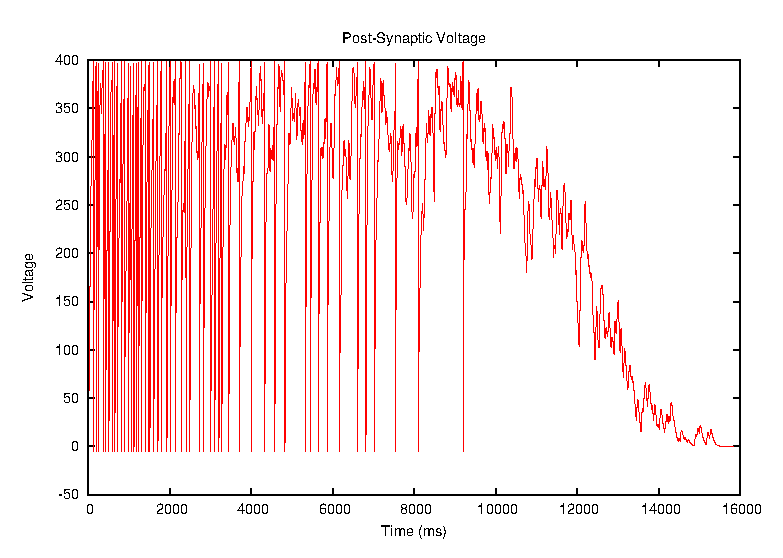
\epsfig{file=data/figures/postSynaptic,width=13cm,height=9cm}
\end{figure}
\end{center}

\begin{center}
\begin{figure}[ht!]
\epsfig{file=data/figures/postTrace,width=13cm,height=9cm}
\epsfig{file=data/figures/postTraceZoom,width=13cm,height=9cm}
\end{figure}
\end{center}

\begin{center}
\begin{figure}[ht!]
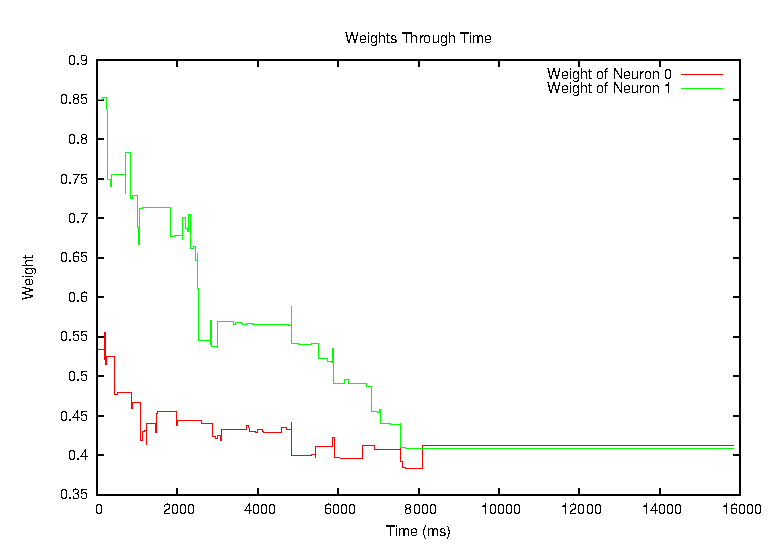
\epsfig{file=data/figures/weightsThroughTime,width=13cm,height=9cm}
\epsfig{file=data/figures/allWeights,width=13cm,height=9cm}
\end{figure}
\end{center}

\end{document}
